\documentclass[a4paper, openany]{memoir}

\usepackage[utf8]{inputenc}
\usepackage[T1]{fontenc} 
\usepackage[english]{babel}
\usepackage{fancyhdr}
\usepackage{float}
\usepackage{amsmath}
\usepackage{amsthm}
\usepackage{amssymb}
\usepackage{enumitem}
\usepackage[bookmarksopen=true,bookmarksopenlevel=2]{hyperref}
\usepackage{tikz}
\usepackage{pgfplots}
\usepackage{indentfirst}
\usepackage{bm}

\pagestyle{fancy}
\fancyhf{}
\fancyhead[LE]{\leftmark}
\fancyhead[RO]{\rightmark}
\fancyhead[RE, LO]{3H CA}
\fancyfoot[LE, RO]{\thepage}
\fancyfoot[RE, LO]{Pete Gautam}

\renewcommand{\headrulewidth}{1.5pt}

\theoremstyle{definition}
\newtheorem{definition}{Definition}[section]

\theoremstyle{plain}
\newtheorem{theorem}[definition]{Theorem}
\newtheorem{lemma}[definition]{Lemma}
\newtheorem{proposition}[definition]{Proposition}
\newtheorem{corollary}[definition]{Corollary}
\newtheorem{example}[definition]{Example}

\chapterstyle{thatcher}
\pgfplotsset{compat=newest}
\setcounter{chapter}{1}

\begin{document}
\chapter{Complex integration}
\section{Introduction to complex integration}
We can define integration in the complex plane in a similar way to line integration in $\mathbb{R}^2$. We integrate over paths. We start by defining paths.
\begin{definition}
Let $\Omega \subseteq \mathbb{C}$ be open, and let $\gamma: [a, b] \to \mathbb{C}$ be a function. We say that $\gamma$ is a \emph{path} if $\gamma$ is continuously differentiable.
\end{definition}
\noindent We can define integration by breaking an integral into real and imaginary part. That is, if $\gamma: [a, b] \to \Omega$ is a path and $f: \Omega \to \mathbb{C}$ is a function, then we define
\begin{align*}
    \int_\gamma f(z) \ dz &= \int_\gamma (u(x, y) + iv(x, y)) \ (dx + idy) \\
    &= \int_\gamma (u(x, y) \ dx - v(x, y) \ dy) + i \int_\gamma (v(x, y) \ dx + u(x, y) \ dy).
\end{align*}
This is called the complex contour integral.

The integrals themselves are defined by Riemann sums. For a path $\gamma: [a, b] \to \Omega$, we can partition $[a, b]$ into small intervals
\[[a_0, a_1], [a_1, a_2], \dots, [a_{n-1}, a_n],\]
where $a_0 < a_1 < \dots < a_n$. The corresponding Riemann sum is
\[\sum_{r=1}^n f(\gamma(t_r)) \cdot (\gamma(a_r) - \gamma(a_{r-1}))\]
for some $t_r \in (a_{r-1}, a_r)$. In the real case, we have chosen: left and right values or suprema and infima as a possible $t_r$. 

We will now define contour integral.
\begin{definition}
Let $f: \Omega \to \mathbb{C}$ be continuous and $\gamma: [0, 1] \to \Omega$ be a path in $\Omega$. Then, the contour integral of $f$ along $\gamma$ is the limit
\[\int_\gamma f(z) \ dz = \lim_{n \to \infty} \sum_{r=1}^n f(\gamma(t_r)) (\gamma(\tfrac{r}{n}) - \gamma(\tfrac{r-1}{n}))\]
for some $t_r \in (\tfrac{r-1}{n}, \tfrac{r}{n})$.
\end{definition}
\noindent Because $f$ is continuous, the limit does not depend on the choice of $t_r$. 

Travelling in the other direction would make the integral negative.
\begin{proposition}
Let $\gamma: [0, 1] \to \Omega$ be a path and let $f: \Omega \to \mathbb{C}$ be a function. Define the function $\overline{\gamma}: [0, 1] \to \Omega$ by $\overline{\gamma}(t) = \gamma(1-t)$. Then,
\[\int_{\overline{\gamma}} f(z) \ dz = -\int_\gamma f(z) \ dz.\]
\end{proposition}

We can also bound integrals.
\begin{proposition}
Let $\gamma: [0, 1] \to \Omega$ be a path of finite length, i.e.
\[\int_0^1 |\gamma'(t)| \ dt \leq L,\]
for some $L \in \mathbb{R}$, and let $f: \Omega \to \mathbb{C}$ be bounded on $\gamma([0, 1]) \subseteq \Omega$, i.e.
\[|f(z)| \leq M\]
for all $z \in \gamma([0, 1])$. Then,
\[\left|\int_\gamma f(z) \ dz\right| \leq ML.\]
\end{proposition}
\begin{proof}
For all $n \in \mathbb{Z}_{\geq 1}$, we have
\begin{align*}
    \left|\sum_{r=1}^n f(\gamma(t_r)) (\gamma(a_r) - \gamma(a_{r-1}))\right| &\leq \sum_{r=1}^n |f(t_r)| |\gamma(a_r) - \gamma(a_{r-1})| \\
    &\leq M \sum_{r=1}^n |\gamma(a_r) - \gamma(a_{r-1})| \leq ML.
\end{align*}
By the order property of limits, this implies that
\[\left|\int_\gamma f(z) \ dz\right| \leq ML.\]
\end{proof}

We now define a curve.
\begin{definition}
Let $\gamma: [0, 1] \to \Omega$ be a function. Then, we say that $\gamma$ is a \emph{curve} if $\gamma$ is continuously differentiable except for finitely many points.
\end{definition}
\noindent We will refer to curves as paths as well. 

For continuous functions, there is a much simpler way to characterise their integrals.
\begin{proposition}
Let $\gamma: [0, 1] \to \Omega$ be a curve of finite length. Then, for any continuous function $f: \Omega \to \mathbb{C}$, we find that
\[\int_\gamma f(z) \ dz = \int_0^1 f(\gamma(t)) \gamma'(t) \ dt.\]
\end{proposition}
\noindent The variable $t \in \mathbb{R}$, but the integrand by itself need not be real. We illustrate how to use this with an example.
\begin{example}
Let $\gamma: [\alpha, \beta] \to \mathbb{C}$ be the path given by $\gamma(\theta) = c + re^{i \theta}$, for $c \in \mathbb{C}$ and $r > 0$. Then, the length of $\gamma$ is given by
\[\int_\alpha^\beta |\gamma'(\theta)| \ d\theta = r(\beta - \alpha).\]
\end{example}
\begin{proof}
We have $\gamma'(\theta) = ire^{i \theta}$. Then, the length of $\gamma$ is:
\begin{align*}
    \int_\alpha^\beta |\gamma'(\theta)| \ d\theta &= \int_\alpha^\beta |ir e^{i \theta}| \ d\theta \\
    &= \int_\alpha^\beta r \ d\theta =  r(\beta - \alpha).
\end{align*}
\end{proof}
Next, we compute an integral.
\begin{example}
Let $\gamma: [\alpha, \beta] \to \mathbb{C}$ be the path given by
\[\gamma(t) = e^{it},\]
and let $n \in \mathbb{Z}$. Then,
\[\int_\gamma z^n \ dz = \begin{cases}
i(\beta - \alpha) & n = -1 \\
\frac{e^{i\beta(n+1)} - e^{i\alpha(n+1)}}{n+1} & \text{otherwise}.
\end{cases}\]
\end{example}
\begin{proof}
Let $f: \mathbb{C} \to \mathbb{C}$ be given by $f(z) = z^n$. We have $\gamma'(t) = ie^{it}$. 
In that case,
\begin{align*}
    \int_\gamma z^n \ dz &= \int_\alpha^\beta f(\gamma(t)) \gamma'(t) \ dt \\
    &= \int_\alpha^\beta (e^{it})^n \cdot ie^{it} \ dt \\
    &= \int_\alpha^\beta ie^{it(n+1)} \ dt.
\end{align*}
Now, if $n = -1$, then
\[\int_\gamma z^{-1} \ dz = \int_\alpha^\beta i \ dt = i(\beta - \alpha).\]
Instead, if $n \neq 1$, then
\[\int_\gamma z^n \ dz = \int_\alpha^\beta ie^{it(n+1)} \ dt = \left[\frac{ie^{it(n+1)}}{i(n+1)}\right]_\alpha^\beta = \frac{e^{i\beta(n+1)} - e^{i\alpha(n+1)}}{n+1}.\]
\end{proof}
\noindent In particular, if $\alpha = 0$ and $\beta = 2\pi$, then
\[\int_\gamma z^{-1} \ dz = 2\pi i,\]
and for $n \neq 1$,
\[\int_\gamma z^n \ dz = \frac{1 - 1}{n+1} = 0.\]

The following is the complex version of the fundamental theorem of calculus.
\begin{proposition}
Let $\Omega \subseteq \mathbb{C}$ be open, and let $f: \Omega \to \mathbb{C}$ be continuous. If there exists a holomorphic function $F: \Omega \to \mathbb{C}$ such that $F' = f$, then for any path $\gamma: [0, 1] \to \Omega$, we have
\[\int_\gamma f(z) \ dz = F(\gamma(1)) - F(\gamma(0)).\]
\end{proposition}
\begin{proof}
Using the complex chain rule, we know that
\[\frac{d}{dt}F(\gamma(t)) = F'(\gamma(t)) \gamma'(t).\]
Therefore,
\begin{align*}
    \int_\gamma f(z) \ dz &= \int_0^1 f(\gamma(t)) \gamma'(t) \\
    &= \int_0^1 \frac{d}{dt} F(\gamma(t)) \ dt \\
    &= F(\gamma(1)) - F(\gamma(0))
\end{align*}
using the real version of the fundamental theorem of calculus.
\end{proof}

This gives us the following consequence.
\begin{corollary}
Let $\gamma: [0, 1] \to \Omega$ be a closed path (i.e. $\gamma(0) = \gamma(1)$), and let $f: \Omega \to \mathbb{C}$ be continuous with antiderivative $F$. Then,
\[\int_\gamma f(z) \ dz = 0.\]
\end{corollary}
We know that for a polynomial, we can integrate it termwise. In particular, if
\[f(z) = \sum_{n=0}^{\alpha} a_n z^n,\]
then
\[\int f(z) \ dz = k + \sum_{n=0}^\alpha \frac{a_n}{n+1} z^{n+1}.\]
So, for a closed path, the integral is 0. We can use this to show that $z \mapsto \frac{1}{z}$ does not have an anti-derivative.
\begin{example}
The holomorphic function $f: \mathbb{C}^\times \to \mathbb{C}$ given by $f(z) = \frac{1}{z}$ does not have an anti-derivative.
\end{example}
\begin{proof}
Let $\gamma: [0, 1] \to \mathbb{C}^\times$ be a path given by $\gamma(t) = e^{2\pi it}$. We know that
\[\int_\gamma f(z) \ dz = i(2\pi - 0) = 2\pi i.\]
We know that $\gamma(0) = 1 = \gamma(1)$. So, the result above tells us that $f$ does not have an anti-derivative.
\end{proof}

\newpage

\section{Cauchy's Theorem}
Previously, we saw that if a function has an antiderivative, then its integral over any closed path is 0. In this section, we will generalise this to holomorphic functions. Moreover, we will look at some applications of this theorem.

Before generalising, we define a simple path.
\begin{definition}
Let $\gamma: [a, b] \to \mathbb{C}$ be a path. Then, $\gamma$ is \emph{simple} if the restriction of $\gamma$ to $(a, b)$ is injective.
\end{definition}
\noindent Intuitively, this means that the path doesn't cross itself except perhaps at the end. For a simple closed path, we can uniquely label any point $z \in \mathbb{C}$ to either be inside $\gamma$ or outside $\gamma$. For example, consider the following path below.
\begin{figure}[H]
    \centering
    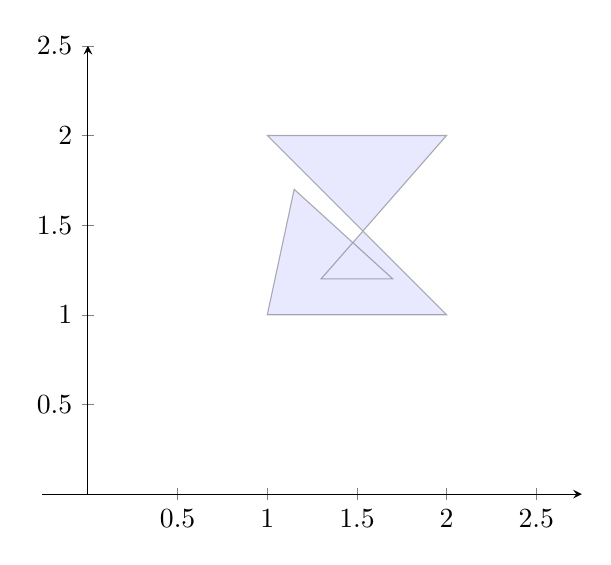
\begin{tikzpicture}
        \begin{axis}[
            axis equal,
            axis lines=center,
            xmin=0, xmax=2.5,
            ymin=0, ymax=2.5
        ]
            \draw[fill=blue!30, opacity=0.3] (1, 1) -- (2, 1)
                -- (1, 2)
                -- (2, 2)
                -- (1.3, 1.2)
                -- (1.7, 1.2)
                -- (1.15, 1.7)
                -- cycle;
        \end{axis}
    \end{tikzpicture}
\end{figure}
\noindent This is not a simple path since it crosses over itself multiple times. However, the following path is simple.
\begin{figure}[H]
    \centering
    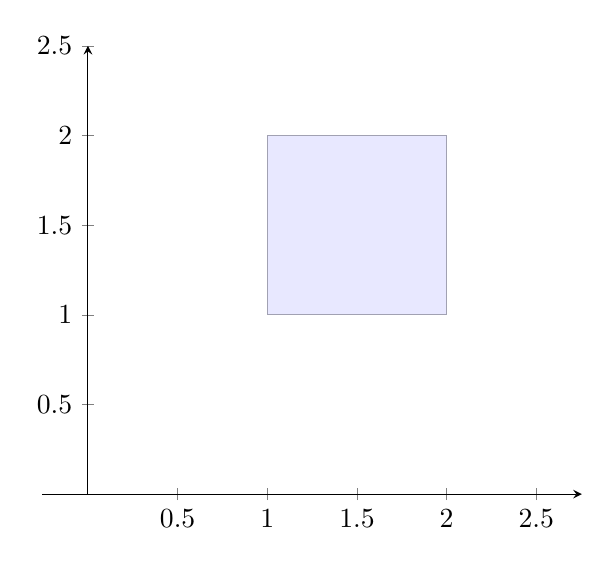
\begin{tikzpicture}
        \begin{axis}[
            axis equal,
            axis lines=center,
            xmin=0, xmax=2.5,
            ymin=0, ymax=2.5
        ]
            \draw[fill=blue!30, opacity=0.3] (1, 1) rectangle (2, 2);
        \end{axis}
    \end{tikzpicture}
\end{figure}
\noindent Clearly, the path doesn't cross over itself, except at the edges.

Below is Cauchy's Theorem- the generalisation to holomorphic functions. 
\begin{theorem}[Cauchy's Theorem]
Let $f: \Omega \to \mathbb{C}$ be a holomorphic function, and let $\gamma: [a, b] \to \Omega$ be a simple closed path such that all points inside $\gamma$ are in $\Omega$. Then,
\[\oint_\gamma f(z) \ dz = 0.\]
\end{theorem}
We prove Cauchy's Theorem in two steps. First, we only consider contours $\gamma$ which are images of rectangles.
\begin{lemma}
Let $f: \Omega \to \mathbb{C}$ be holomorphic. Let $R = [0, 1] \times [a, b]$ be a rectangle in $\mathbb{R}^2$ with boundary $\partial R$ and $\gamma: \partial R \to \Omega$ be a path such that $\gamma = \Gamma|_{\partial R}$ for some continuous function $\Gamma: R \to \Omega$. Then,
\[\oint_\gamma f(z) \ dz = 0.\]
\end{lemma}
\begin{proof}
Let
\[I(R) = \left|\oint_{\gamma(R)} f(z) \ dz\right|.\]
Define the sequence $(R_i)_{i=1}^\infty$ where $R_1$ is a quarter of $R$, and $R_i$ is a quarter of $R_{i+1}$. We illustrate $R$ (red), $R_1$ (blue) and $R_2$ (green) in the figure below.
\begin{figure}[H]
    \centering
    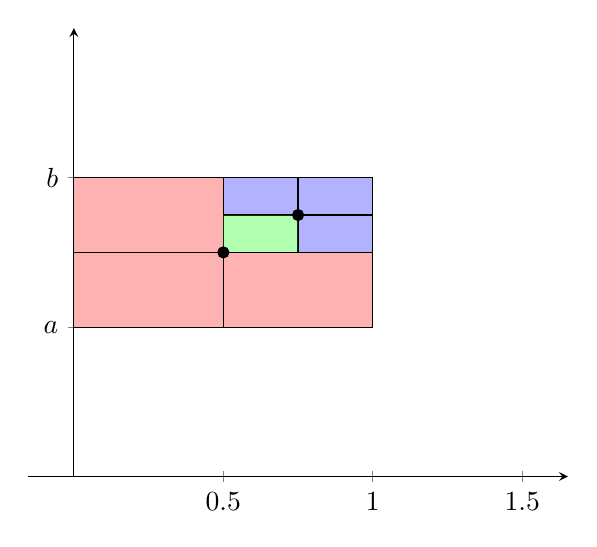
\begin{tikzpicture}
        \begin{axis}[
            axis equal,
            xmin=0, xmax=1.5,
            ymin=0, ymax=1.5,
            axis lines=center,
            ytick={0.5, 1},
            yticklabels={$a$, $b$},
        ]
            \draw[fill=red, opacity=0.3] (0, 0.5) -- (1, 0.5)
                -- (1, 0.75)
                -- (0.5, 0.75)
                -- (0.5, 1)
                -- (0, 1)
                -- cycle;

            \draw[fill=blue, opacity=0.3] (0.75, 0.875) -- (0.75, 0.75)
                -- (1, 0.75)
                -- (1, 1)
                -- (0.5, 1)
                -- (0.5, 0.875)
                -- cycle;
            \draw (0, 0.5) rectangle (1, 1);
            \draw (0, 0.75) -- (1, 0.75); 
            \draw (0.5, 0.5) -- (0.5, 1);

            \draw (0.5, 0.875) -- (1, 0.875); 
            \draw (0.75, 0.75) -- (0.75, 1);

            \draw[fill=green, opacity=0.3] (0.75, 0.875) rectangle (0.5, 0.75);

            \draw[fill] (0.5, 0.75) circle (2pt);
            \draw[fill] (0.75, 0.875) circle (2pt);
        \end{axis}
    \end{tikzpicture}
\end{figure}
\noindent Note that the choices of $R_1$ and $R_2$ is not unique.

The rectangle has area $I(R_i)$ for some $i \in \mathbb{Z}_{\geq 1}$. Moreover, the opposite edges on the boundary are of the same size and have opposite orientations with respect to the path $\gamma$. In that case, we find that
\[I(R) \leq 4I(R_1) \leq 4^2 I(R_2) \leq \dots\]
by the integral version of the triangle inequality.

So, for all $n \in \mathbb{Z}_{\geq 1}$, $I(R) \leq 4^n I(R_n)$. Moreover, we get a sequence of points $(s_n)_{n=1}^{\infty}$ and $(t_n)_{n=1}^\infty$ in $\mathbb{R}$ that lie at the intersection of the rectangles (as shown in the figure above). Then, by construction, the values converge in $\mathbb{R}$ to $s$ and $t$ respectively. Set $w = \Gamma(s, t)$. Since $\Gamma$ is continuous, the sequence $w_n = \Gamma(s_n, t_n)$ converges to $w$. Moreover, $f$ is differentiable at $w \in \Gamma(R) \subseteq \Omega$, so
\[f(z) = f(w) + f'(w)(z - w) + q(z) (z - w)\]
for $z \in \Omega \setminus \{w\}$, where 
\[q(z) = \frac{f(z) - f(w)}{z - w} - f'(w).\]
If we set $q(w) = 0$ along with the definition above, $q: \Omega \to \mathbb{C}$ is continuous. This is because
\[\lim_{z \to w} q(z) = \lim_{z \to w} \left[\frac{f(z) - f(w)}{z - w} - f'(w)\right] = f'(w) - f'(w) = 0.\]
In that case, for $n \in \mathbb{Z}_{\geq 1}$,
\begin{align*}
    I(R_n) &= \oint_{\gamma(R_n)} f(z) \ dz \\
    &= \oint_{\gamma(R_n)} f(w) + f'(w) (z - w) + q(z) (z - w) \ dz \\
    &= \oint_{\gamma(R_n)} q(z) (z - w) \ dz
\end{align*}
since the functions $z \mapsto f(w)$ and $z \mapsto f'(w) (z - w)$ have anti-derivatives and $\gamma(R_n)$ is a closed path.

\noindent The side lengths of $R_n$ are given by $2^{-n} R$. Moreover, we can choose $\Gamma: R \to \Omega$ such that lengths in $R$ get scaled by a finite amount when mapped to $\Omega$ under $\Gamma$. Therefore, there exist constants $K, L > 0$ such that the length of $\Gamma(R_n)$ is given by
\[\Gamma|_{\partial R_n} \leq 2^{-n} K,\]
and
\[|z - w| \leq 2^{-n}L\]
for all $z \in \gamma(R_n) = \Gamma|_{\partial R_n}$.
Moreover, since $q(z) \to 0$ as $z \to w$, it must be bounded. So, for all $n \in \mathbb{Z}_{\geq 1}$, there exists an $M_n > 0$ such that $|q(z)| \leq M_n$ for all $z \in \gamma(R_n)$. In that case,
\begin{align*}
    0 \leq I(R) &\leq 4^n I(R_n) \\
    &\leq 4^n \oint |q(z) (z - w)| \ dz \\
    &\leq 4^n \cdot 2^{-n}K \cdot 2^{-n} L \cdot M_n \\
    &= KL M_n.
\end{align*}
Since $q(z) \to 0$ as $z \to w$, we can choose $M_n \to 0$. Therefore, 
\[I(R) = \left|\oint_\gamma f(z) \ dz\right| = 0.\]
This implies that
\[\oint_\gamma f(z) \ dz = 0.\]
\end{proof}

Now, we will use this result to show that Cauchy's Theorem holds for all simple closed paths. For this, we define homotopy.
\begin{definition}
Let $\gamma, \delta: [a, b] \to \Omega$ are called \emph{homotopic} if there exists a continuous function $\Gamma: [0, 1] \times [a, b] \to \Omega$, called a \emph{homotopy} from $\gamma$ to $\delta$, such that
\begin{itemize}
    \item $\Gamma(s, a) = \gamma(a) = \delta(a)$ and $\Gamma(s, b) = \gamma(b) = \delta(b)$ for all $s \in [0, 1]$, and
    \item $\Gamma(0, t) = \gamma(t)$ and $\Gamma(1, t) = \delta(t)$ for all $t \in [a, b]$.
\end{itemize}
\end{definition}
\noindent The following is an example of two paths $\gamma$ and $\delta$ that are homotopic.
\begin{figure}[H]
    \centering
    \begin{tikzpicture}
        \begin{axis}[
            axis equal,
            axis lines=center,
            xmin=0, xmax=0.75,
            ymin=0, ymax=0.8,
        ]
            \draw[blue] (0.5, 0.2) -- (0.5, 0.7);
            \draw[red] (0.5, 0.7) arc (90:270:0.25);
            \node at (0.55, 0.45) {$\delta$};
            \node at (0.2, 0.45) {$\gamma$};

            \draw[thick, dotted] (0.5, 0.2) to[bend left=15] (0.5, 0.7);
            \draw[thick, dotted] (0.5, 0.2) to[bend left=45] (0.5, 0.7);
            \draw[thick, dotted] (0.5, 0.2) to[bend left=90] (0.5, 0.7);
        \end{axis}
    \end{tikzpicture}
\end{figure}
\noindent The dotted lines represent the deformations that we can take going from $\gamma$ to $\delta$. Informally, for two paths to be homotopic, it means that we can continuously deform one into another, as shown above.

For a point $w \in \Omega$, the trivial path $\delta: [a, b] \to \Omega$ is the path where $\delta(t) = w$ for all $t \in [a, b]$. If a path $\gamma: [a, b] \to \Omega$ is homotopic to $\delta$ (for some $w \in \Omega$), then we say that it is \emph{null-homotopic}.

Next, we show that the contour integral over closed homotopic paths is equal.
\begin{lemma}
Let $f: \Omega \to \mathbb{C}$ be holomorphic and let $\gamma, \delta$ be two closed holomorphic paths in $\Omega$. Then,
\[\oint_\gamma f(z) \ dz = \oint_\delta f(z) \ dz.\]
\end{lemma}
\begin{proof}
Let $\Gamma: [0, 1] \times [a, b] \to \Omega$ be a homotopy from $\gamma$ to $\delta$ in $\Omega$ such that $\gamma(R) = \Gamma|_{\partial R}$ has finite length. Then,
\[\oint_\gamma f(z) \ dz - \oint_\delta f(z) \ dz =  \oint_{\Gamma|_{\partial R}} f(z) \ dz = 0.\]
% TODO: Illustrate with an image
\end{proof}
Using this lemma, we can show that if a path is null-homotopic, it satisfies the Cauchy's Theorem.
\begin{proposition}
Let $f: \Omega \to \mathbb{C}$ be holomorphic and $\gamma$ be a null-homotopic path in $\Omega$. Then,
\[\oint_\gamma f(z) \ dz = 0.\]
\end{proposition}
\begin{proof}
Let $\delta: [a, b] \to \mathbb{C}$ be the path given by $\delta(t) = \gamma(a) = \gamma(b)$. Then,
\[\oint_\gamma f(z) \ dz = \oint_\delta f(z) \ dz = \int_a^b f(\delta(t)) \delta'(t) \ dt = 0.\]
\end{proof}
\noindent In Cauchy's Theorem, we require a path $\gamma$ to be simple. This property is enough for a path to be null-homotopic in $\Omega$ since it can be shrunk into a point inside $\Omega$ without obstructions.

Using Cauchy's Theorem, we can provide Cauchy's Integral Formula.
\begin{proposition}[Cauchy's Integral Formula]
Let $f: \Omega \to \mathbb{C}$ be a holomorphic function, and let $\gamma: [0, 1] \to \Omega$ be a simple closed path traced anticlockwise. Then,
\[f(z) = \frac{1}{2\pi i} \oint_\gamma \frac{f(\zeta)}{\zeta - z} \ d\zeta\]
for all $z \in \Omega$ that lie in $\gamma$.
\end{proposition}
\begin{proof}
Let $z \in \Omega$. Since $\Omega$ is open, there exists an open disc $D$ of radius $r$ around $z$ that is contained in $\Omega$. Then, let $\varepsilon \in (0, r)$ and $\delta_\varepsilon$ be a circle of radius $\varepsilon$ with center at $z$. This is illustrated below.
\begin{figure}[H]
    \centering
    \begin{tikzpicture}
        \begin{axis}[
            axis equal,
            axis lines=center,
            xmin=0, xmax=2,
            ymin=0, ymax=2,
            xticklabels={}, yticklabels={},
        ]
            \draw plot [smooth cycle] coordinates {(0.5, 1) (1, 0.5) (1.5, 0.5) (1.5, 1.5) (0.7, 1.5) (1.25, 1)};

            \filldraw (1.25, 0.75) circle (1pt);
            \node at (1.3, 0.75) {$z$};
            \draw[red] (1.25, 0.75) circle (0.15);
            
            \node at (1, 0.4) {$\gamma$};
            \node at (1, 0.7) {$\delta_\varepsilon$};
        \end{axis}
    \end{tikzpicture}
\end{figure}
\noindent Clearly, $\gamma$ is homotopic to $\delta$ in $\Omega \setminus \{z\}$. In that case,
\[\oint_\gamma \frac{f(\zeta)}{\zeta - z} \ d\zeta = \oint_{\delta_\varepsilon} \frac{f(\zeta)}{\zeta - z} \ d\zeta.\]
So,
\[\left|\oint_{\delta_\varepsilon} \frac{f(\zeta)}{\zeta - z} \ d\zeta - \oint_{\delta_\varepsilon} \frac{f(z)}{\zeta - z} \ d\zeta\right| = \left|\oint_{\delta_\varepsilon} \frac{f(\zeta) - f(z)}{\zeta - z} \ d\zeta\right| < 2\pi \varepsilon (|f'(z)| + 1).\]
The length of the path is $2\pi \varepsilon$, since $\varepsilon$ is the radius of the circle. Moreover, since
\[\frac{f(\zeta) - f(z)}{\zeta - z} \to f'(z),\]
we can bound the integrand by $|f'(z)| + 1$ for all $\varepsilon \leq \varepsilon'$, where $\varepsilon' \in (0, r)$. As $\varepsilon \to 0$, we find that
\[\left|\oint_{\delta_\varepsilon} \frac{f(\zeta)}{\zeta - z} \ d\zeta - \oint_{\delta_\varepsilon} \frac{f(z)}{\zeta - z} \ d\zeta\right| \to 0.\]
Moreover, we find that
\begin{align*}
    \oint_{\delta_\varepsilon} \frac{f(z)}{\zeta - z} \ d\zeta &= f(z) \oint_{\delta_\varepsilon} \frac{d\zeta}{\zeta - z} \\
    &= f(z) \int_0^{2\pi} \frac{1}{z + \varepsilon e^{it} - z} \cdot i \varepsilon e^{it} \ dt \\
    &= f(z) \int_0^{2\pi} \frac{i \varepsilon e^{it}}{\varepsilon e^{it}} \ dt \\
    &= 2\pi i f(z).
\end{align*}
In that case,
\[\oint_\gamma \frac{f(\zeta)}{\zeta - z} \ d\zeta = \oint_{\delta_\varepsilon} \frac{f(\zeta)}{\zeta - z} \ d\zeta = \oint_{\delta_\varepsilon} \frac{f(z)}{\zeta - z} \ d\zeta = 2\pi i f(z).\]
So,
\[f(z) = \frac{1}{2\pi i} \oint_\gamma \frac{f(\zeta)}{\zeta - z} \ d\zeta\]
\end{proof}

We can generalise this even further and compute the derivatives by integrating.
\begin{proposition}
Let $f: \Omega \to \mathbb{C}$ be a holomorphic function, and let $\gamma: [0, 1] \to \Omega$ be a simple closed path traced anticlockwise. Then, $f$ is infinitely differentiable on $\Omega$, with
\[f^{(n)}(z) = \frac{n!}{2\pi i} \oint_\gamma \frac{f(\zeta)}{(\zeta - z)^{n+1}} \ d\zeta\]
for $z \in \Omega$ that lies in $\gamma$ and $n \in \mathbb{Z}_{\geq 0}$.
\end{proposition}
\begin{proof}
We prove this by induction. We know that if $n = 0$, then the statement is the Cauchy's Integral Formula. So, now assume that $f$ is $n$-differentiable on $\Omega$ with
\[f^{(n)}(z) = \frac{n!}{2\pi i} \oint_\gamma \frac{f(\zeta)}{(\zeta - z)^{n+1}} \ d\zeta\]
for $z \in \Omega$. Then,
\begin{align*}
    f^{(n+1)}(z) &= \frac{d}{dz} f^{(n)}(z) \\
    &= \frac{n!}{2\pi i} \oint_\gamma \frac{d}{dz} \frac{f(\zeta)}{(\zeta - z)^{n+1}} \ d\zeta \\
    &= \frac{n!}{2\pi i} \oint_\gamma \frac{(n+1) f(\zeta)}{(\zeta - z)^{n+2}} \ d\zeta \\
    &= \frac{(n+1)!}{2\pi i} \oint_\gamma \frac{f(\zeta)}{(\zeta - z)^{n+2}} \ d\zeta.
\end{align*}
So, the statement follows from induction.
\end{proof}
\noindent This theorem tells us that a function that can be differentiable once can be infinitely differentiated. This is not true in real analysis.

Using this result, we can show that holomorphic functions are locally analytic.
\begin{proposition}
Let $f: \Omega \to \mathbb{C}$ be a holomorphic function. Then, for all $c \in \Omega$, there exists an open disc $D_c \subseteq \Omega$ with center $c$ such that
\[f(z) = \sum_{n=0}^\infty \frac{f^{(n)}(c)}{n!} (z - c)^n\]
for all $z \in D_c$.
\end{proposition}
\begin{proof}
Let $c \in \Omega$. Since $\Omega$ is open, there exists an open disc $D_C$ centered at $c$ such that $D_c \subseteq \Omega$. Now, let $z \in D_C$, and let $\gamma$ be a closed circle with center $c$ containing $z$. Then,
\[\sum_{n=0}^\infty \frac{f^{(n)}(c)}{n!} (z - c)^n = \frac{1}{2\pi i} \sum_{n=0}^\infty \oint_\gamma \frac{f(\zeta) (z - c)^n}{(\zeta - c)^{n-1}} \ d\zeta\]
using Cauchy's integral formula for derivatives. Moreover, the power series
\[\sum_{n=0}^\infty \frac{f(\zeta) (z - c)^n}{(\zeta - c)^{n+1}} = \frac{f(\zeta)}{\zeta - c} \sum_{n=0}^\infty \frac{(z - c)^n}{(\zeta - c)^n} = \frac{f(\zeta)}{\zeta - z}\]
since
\[\frac{|z - c|}{|\zeta - c|} < 1.\sidefootnote{The value $\zeta$ lies at the boundary of $D_c$, whereas the value $z$ lies inside $D_c$.}\]
This implies that
\begin{align*}
    \sum_{n=0}^\infty \frac{f^{(n)}(c)}{n!} (z - c)^n &= \frac{1}{2\pi i} \oint_\gamma \sum_{n=0}^\infty \frac{f(\zeta)}{(\zeta - c)^{n-1}} \  d\zeta \cdot (z - c)^n \\
    &= \frac{1}{2\pi i} \oint_\gamma \frac{f(\zeta)}{\zeta - z} \ d\zeta = f(z)
\end{align*}
using Cauchy's formula.
\end{proof}

We can use Cauchy's integral formula to prove Lioville's Theorem.
\begin{theorem}[Lioville's Theorem]
Let $f: \mathbb{C} \to \mathbb{C}$ be a holomorphic function that is not a constant. Then, $f$ is not bounded.
\end{theorem}
\begin{proof}
We prove this by contrapositive. So, assume that $f$ is bounded. In that case, there exists an $M > 0$ such that for all $z \in \mathbb{C}$, $|f(z)| \leq M$. We show that $f$ is a constant. Let $z \in \mathbb{C}$ and $r > 0$. Define the path $\gamma: [0, 2\pi] \to \mathbb{C}$ by $\gamma(t) = z + re^{it}$. By Cauchy's Integral Formula, we find that
\[f'(z) = \frac{1}{2\pi i} \oint_\gamma \frac{f(\zeta)}{(z - \zeta)^2} \ d\zeta.\]
We know that $|f(\zeta)| \leq M$ for all $\zeta \in \gamma$. Moreover, for all $\zeta \in \gamma$, $|z - \zeta| = r$. In that case,
\[\left|\oint_\gamma \frac{f(\zeta)}{(z - \zeta)^2}\right| \leq 2\pi r \cdot \frac{M}{r^2} = \frac{2M \pi}{r}.\]
So, we find that
\[|f'(z)| = \frac{1}{2\pi} \left|\oint_\gamma \frac{f(\zeta)}{(z - \zeta)^2} \ d\zeta\right| \leq \frac{M}{r}\]
for all $r > 0$. This implies that $f'(z) = 0$. So, $f$ is a constant.
\end{proof}
\noindent Using this theorem, we can prove the Fundamental Theorem of Algebra.
\begin{theorem}[Fundamental Theorem of Algebra]
Let $p: \mathbb{C} \to \mathbb{C}$ be a polynomial in $\mathbb{C}$ of degree at least 1. Then, $p$ has a root in $\mathbb{C}$.
\end{theorem}
\begin{proof}
Assume, for a contradiction, that $p$ has no root in $\mathbb{C}$. In that case, for all $z \in \mathbb{C}$, $p(z) \neq 0$. This implies that the reciprocal function $f: \mathbb{C} \to \mathbb{C}$ given by $f(z) = \frac{1}{p(z)}$ is holomorphic. Moreover, since $p$ is of degree at least 1, $p$ is not bounded. So, $f(z) \to 0$ as $|z| \to \infty$. This implies that $|f(z)| \leq K$ for all $|z| > L$. Now, define the path $\gamma:[0, 2\pi] \to \mathbb{C}$ by $\gamma(t) = z + Re^{it}$, for $R > |z| + L$. This is illustrated below.
\begin{figure}[H]
    \centering
    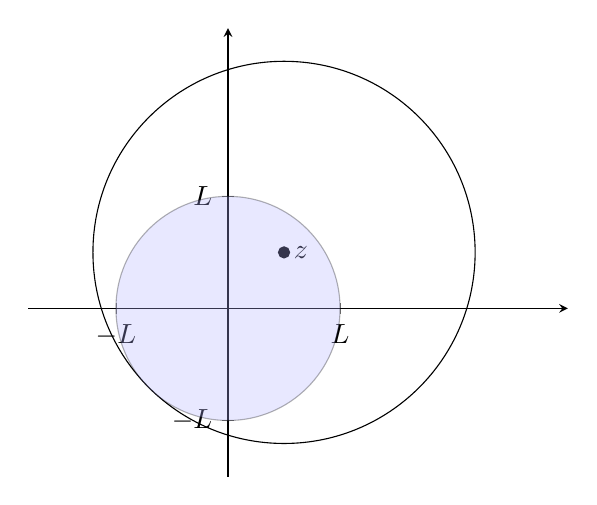
\begin{tikzpicture}
        \begin{axis}[
            axis equal,
            axis lines=center,
            xmin=-2.5, xmax=5,
            ymin=-3, ymax=5,
            xticklabels={$-L$, $L$}, xtick={-2, 2},
            yticklabels={$-L$, $L$}, ytick={-2, 2},
        ]
            \filldraw (1, 1) circle (2pt);
            \node at (1.3, 1) {$z$};

            \draw (1, 1) circle (2 + 1.41);
            \draw[fill=blue!30, opacity=0.3] (0, 0) circle (2);
        \end{axis}
    \end{tikzpicture}
\end{figure}
\noindent By construction, we find that $|\gamma(t)| > L$ for all $t \in [0, 2\pi]$. In that case, Cauchy's Integral Formula tells us that
\[|f'(z)| = \frac{1}{2\pi} \left|\oint_\gamma \frac{f(\zeta)}{(\zeta - z)^2} \ d\zeta\right| \leq \frac{1}{2\pi} \cdot 2\pi r \cdot \frac{K}{r^2} = \frac{K}{R}\]
for all $R > |z| + L$. Therefore, $f'(z) = 0$. This means that $f$ is a constant, in which case $p$ too is a constant. This is a contradiction. So, $p$ must have a root in $\mathbb{C}$.
\end{proof}
\noindent Using this theorem, we can show that a polynomial of degree $n$ has $n$ roots in $\mathbb{C}$. Let $p: \mathbb{C} \to \mathbb{C}$ be a polynomial in $\mathbb{C}$ of degree $n \geq 1$. The fundamental theorem of algebra tells us that $p(z) = (z - a)q(z)$, where the degree of $q$ is $n - 1$. If $n - 1 = 0$, then $q$ is a constant, and we have fully factorised $p$. Otherwise, we can start again and find another root for $p$. Continuing $n$ times, we find all the $n$ roots of $p$.
\newpage

\section{Laurent Series}
Let $\Omega \subseteq \mathbb{C}$ be open and $f: \Omega \to \mathbb{C}$ holomorphic. We know that for any $c \in \Omega$, we can find a disc $D_c \subseteq \Omega$ centered at $c$ such that for any $z \in D_c$,
\[f(z) = \sum_{n=0}^\infty a_n (z - c)^n,\]
where
\[a_n = \frac{f^{(n)}(c)}{n!} = \frac{1}{2\pi i} \oint_\gamma \frac{f(\zeta)}{(\zeta - c)^{n+1}} \ d\zeta,\]
where $\gamma \subseteq D_c$ is a circle centered at $c$ and traced anticlockwise.

We can generalise this theorem when $f$ is only holomorphic on $\Omega \setminus \{c\}$ and has a singularity at $z = c$. In such a case, we say that $f$ has an isolated singularity at $c$. The corresponding disc $D_c \subseteq \Omega$ is centered at $c$ still, and $f$ is holomorphic on $D_c \setminus \{c\}$.
\begin{theorem}[Laurent Series]
Let $f: \Omega \setminus \{c\} \to \mathbb{C}$ be holomorphic with $\Omega \subseteq \mathbb{C}$ open and $c \in \Omega$. Then, there exists an open disc $D$ centered at $c$ and $\gamma \subseteq D$ such that
\[f(z) = \sum_{n=-\infty}^{\infty} a_n (z - c)^n,\]
with
\[a_n = \frac{1}{2\pi i} \oint_\gamma \frac{f(\zeta)}{(\zeta - c)^{n+1}} \ d\zeta\]
for all $z \in D \setminus \{c\}$. The expansion of $f$ is called its Laurent series at $c$.
\end{theorem}
\begin{proof}
Let
\[S^+ = \sum_{n=0}^\infty a_n (z - c)^n, \qquad S^- \sum_{n=-\infty}^{-1} a_n (z - c)^n.\]
We show that $f(z) = S^+ + S^-$. Let $\gamma^+$ be a circle with center $c$, where $z$ lies inside $\gamma^+$. We know that
\[\frac{1}{2\pi i} \oint_{\gamma^+} \sum_{n=0}^\infty f(\zeta) \frac{(z- c)^n}{(\zeta - c)^{n+1}} \ d\zeta\]
converges absolutely since
\[\left|\frac{z - c}{\zeta - c}\right| < 1.\]
Therefore,
\begin{align*}
    \frac{1}{2\pi i} \oint_{\gamma^+} \sum_{n=0}^\infty f(\zeta) \frac{(z - c)^n}{(\zeta - c)^{n+1}} &= \sum_{n=0}^\infty \frac{1}{2\pi i} \oint_{\gamma^+} f(\zeta) \frac{(z - c)^n}{(\zeta - c)^{n+1}} \\
    &= \sum_{n=0}^\infty a_n (z - c)^n = S^+.
\end{align*}
We now choose a circle $\gamma^-$ with center $c$ and $z$ outside $\gamma^-$. Then,
\[\left|\frac{\zeta - c}{z - c}\right| < 1,\]
and so
\begin{align*}
    \frac{1}{2\pi i} \oint_{\gamma^-} \sum_{n=0}^\infty f(\zeta) \frac{(\zeta - c)^n}{(\zeta - c)^{n+1}} &= \sum_{n=0}^\infty \frac{1}{2\pi i} \oint_{\gamma^-} f(\zeta) \frac{(\zeta - c)^n}{(z - c)^{n+1}} \ d\zeta \\
    &= \sum_{n=0}^\infty a_{-n-1}(z - c)^{-n-1} = S^-.
\end{align*}
Using the two circles, we define $\delta_\varepsilon$, as shown below.
% TODO: ADD DIAGRAM
The contour $\delta_\varepsilon$ is homotopic to $\gamma^- \cup \gamma^+$ and a connecting line $\lambda$ between the circles $\gamma^-$ and $\gamma^+$. The contribution of the contour integral over $\lambda$ is zero as we integrate twice but with opposite direction of travel. Hence,
\[S^+ + S^- = \oint_{\delta_\varepsilon} \frac{f(\zeta)}{\zeta - z} \ d\zeta.\]
Since $\delta_\varepsilon$ is homotopic to the anticlockwise circle centered at $z$ on $\Omega \setminus \{c\}$, Cauchy's integral formula tells us that $S^+ + S^- = f(z)$.
\end{proof}

Using Laurent series, we can characterise the type of isolated singularities.
\begin{definition}
Let $\Omega \subseteq \mathbb{C}$ be open and $c \in \Omega$, and let $f: \Omega \setminus \{c\} \to \mathbb{C}$ be holomorphic. Then, we call the isolated singularity $c$ of $f$:
\begin{itemize}
    \item a removable singularity if $a_n = 0$ for all $n \leq -1$ in the Laurent expansion.
    \item a finite pole of order $N$ if $a_n = 0$ for all $n \leq -N$ in the Laurent expansion.
    \item an essential singularity if for all $N \in \mathbb{Z}_{\leq 0}$, there exists an $n \in \mathbb{Z}$ with $n \leq N$ and $a_n \neq 0$ in the Laurent expansion.
\end{itemize}
\end{definition}
\noindent If $c$ is a removable singularity, then the Laurent series is an ordinary power series. Moreover, the function $g: \Omega \to \mathbb{C}$
\[g(z) = \begin{cases}
f(z) & z \neq c \\
a_0 & z = c
\end{cases}\]
is holomorphic. Instead, if $c$ is a finite pole of order $N$, then the function
\[f(z) = \sum_{n=-N}^\infty a_n (z - c)^n = \frac{g(z)}{(z - c)^N},\]
for some holomorphic function $g: \Omega \to \mathbb{C}$.

We will now look at the different types of singularities.
\begin{example}
The function $f: \mathbb{C} \setminus \{0\} \to \mathbb{C}$ given by
\[f(z) = \frac{\sin z}{z}\]
has a removable singularity at $z = 0$.
\end{example}
\begin{proof}
We find that
\begin{align*}
    f(z) &= \frac{\sin z}{z} \\
    &= \frac{1}{z} \left(z - \frac{1}{3!}z^3 + \frac{1}{5!} z^5 - \dots\right) \\
    &= 1 - \frac{1}{3!} z^2 + \frac{1}{5!} z^4 - \dots
\end{align*}
Therefore, $f$ is analytic over $\mathbb{C}$. This implies that $f$ is holomorphic on $\mathbb{C}$ if we set $f(0) = 1$. So, $f$ has a removable singularity at $z = 0$.
\end{proof}
\noindent In this case, we have $f(z) \to 1$ as $z \to 0$. So, $|f(z)|$ is bounded on some neighbourhood of $0$.
\begin{example}
The function $g: \mathbb{C} \setminus \{-5, 3\} \to \mathbb{C}$ given by
\[g(z) = \frac{z + 2}{(z - 3)(z + 5)^2}\]
has a pole of order 1 (simple pole) at $z = 3$ and a pole of order 2 (double pole) at $z = -5$.
\end{example}
\noindent In this case, we have $|g(z)| \to \infty$ as $z \to 3$ or $z \to -5$. So, $|g(z)|$ is not bounded on any neighbourhood of $3$ or $-5$.
\begin{example}
The function $h: \mathbb{C} \setminus \{0\} \to \mathbb{C}$
\[h(z) = e^{1/z} = 1  + \frac{1}{z} + \frac{1}{2!} \frac{1}{z^2} + \dots\]
has an isolated essential singularity at $z = 0$.
\end{example}
\noindent In this case, if $z \to 0$ via the positive real values, then $|h(z)| \to \infty$. Instead, if $z \to 0$ through negative real values, then $h(z) \to 0$. So, $h$ is not bounded on any neighbourhood of $0$, but $|h(0)| \not\to \infty$.

We can use the boundedness of neighbourhoods to characterise singularities.
\begin{proposition}
Let $\Omega \subseteq \mathbb{C}$ be open, $c \in \Omega$ and $f: \Omega \setminus \{c\} \to \mathbb{C}$ be holomorphic. Then,
\begin{itemize}
    \item $f$ has a removable singularity at $c$ if and only if $f$ is bounded on some disc $D \subseteq \Omega$ centered at $c$.
    \item $f$ has a pole of finite order at $c$ if and only if $|f(z)| \to \infty$ as $z \to c$.
    \item $f$ has an essential singularity at $c$ if and only if $f$ is unbounded on any neighbourhood of $c$ and $|f(z)| \not\to \infty$ as $z \to c$.
\end{itemize}
\end{proposition}
\begin{proof}
\hspace*{0pt}
\begin{itemize}
    \item Assume first that $f$ has a removable singularity at $c$. Then, $f$ is bounded on a disc centered at $c$. Instead, if $f$ is bounded on a disc $D$ centered at $c$, then $|f(z)| \leq M$ for all $z \in D$. In that case, for $\gamma \subseteq D$ a circle centered at $c$ of radius $r > 0$, we find that for all $n \leq -1$,
    \begin{align*}
        |a_n| &\leq \frac{1}{2\pi} \left|\oint_\gamma \frac{f(\zeta)}{(\zeta - c)^{n+1}} \ d\zeta \right| \\
        &\leq \frac{1}{2\pi} \cdot \frac{M}{r^{n+1}} \cdot 2\pi r = Mr^{-n}.
    \end{align*}
    So, as $r \to 0$, $|a_n| \to 0$. So, $c$ is a removable singularity.
    
    \item Assume now that $f$ has a pole at $c$. Then, $|f(z)| \to \infty$ as $z \to c$. Instead, assume that $|f(z)| \to \infty$ as $z \to c$. Therefore, there must be a disc $D$ centered at $c$ with $|f(z)| > 1$ for all $z \in D$. So, the function $\frac{1}{f}: D \setminus \{c\} \to \mathbb{C}$ is bounded on $D \setminus \{c\}$. This implies that $\frac{1}{f}$ has a removable singularity at $c$. Therefore, $\frac{1}{f(z)} \to 0$ as $z \to c$. So, the Taylor series of $\frac{1}{f}$ must be of the form
    \[\frac{1}{f(z)} = (z - c)^N (a_N + a_{N+1} (z - c) + \dots),\]
    with $a_N \neq 0$ and $N \geq 1$. Therefore, 
    \[\frac{1}{f(z)} = (z - c)^N g(z),\]
    with $g: D \to \mathbb{C}$ holomorphic, and $g(c) \neq 0$. Hence, there is another disc $D'$ around $c$ on which $g(z) \neq 0$. Therefore,
    \[f(z) = (z - c)^{-N} \frac{1}{g(z)},\]
    where $\frac{1}{g}$ is holomorphic on $D'$. So, $f$ has a pole of order $N$ at $c$.
    
    \item If $f$ has an essential singularity at $c$, then $f$ is unbounded on any neighbourhood of $c$ and $|f(z)| \not\to \infty$. Moreover, if $f$ is unbounded and $|f(z)| \to \infty$, then $f$ must have a finite pole. So, if $f$ is unbounded and $|f(z)| \not\to \infty$, then $f$ must have an essential singularity at $c$.
\end{itemize}
\end{proof}
The following is another characterisation of essential singularity.
\begin{theorem}[Casaroti-Weirstrass Theorem]
    Let $\Omega$ be an open set in $\mathbb{C}$, let $c \in \Omega$, and let $f: \Omega \setminus \{c\} \to \mathbb{C}$ be a holomorphic wth an essential singulariy at $c$. Then, the image of any (punctured) disc $D_c$ under $f$ is dense in $\mathbb{C}$. That is, if $w = f(z)$, then the intersection $f(D_c) \cap \overline{D}$ for any disc $\overline{D}$ in the $w$-plane is non-empty.
\end{theorem}

\newpage

\section{Calculus of residues}
We will now look at poles of finite order in more detail. We do this using residues. The following is the definition of the residue.
\begin{definition}
    Let $f: \Omega \setminus \{c\} \to \mathbb{C}$ have an isolated singularity at $c \in \Omega$. Then, the coefficient
    \[a_{-1} = \frac{1}{2\pi i} \oint_\gamma f(z) \ dz\]
    in the Laurent series expansion of $f$ at $c$ is called the \emph{residue of $f$ at $c$}. It is denoted $\operatorname{res}(f, c)$. Here, $\gamma$ is a circle centered at $c$ and traced anti-clockwise.
\end{definition}

We will generalise Cauchy's Theorem for functions with isolated singularities.
\begin{theorem}[Cauchy's Residue Theorem]
    Let $\Omega \subseteq \mathbb{C}$ be open and $c_1, \dots, c_k \in \Omega$ be finitely many points at which $f: \Omega \setminus \{c_1, \dots, c_k \} \to \mathbb{C}$ is not holomorphic. For any simple closed path $\gamma \subseteq \Omega$ such that $c_1, \dots, c_k$ lie inside $\gamma$, we have
    \[\oint_\gamma f(z) \ dz = 2\pi i \sum_{n=1}^k \operatorname{res}(f, c_n).\]
\end{theorem}
\begin{proof}
    The path $\gamma$ is homotopic to the path $\delta_\varepsilon$ shown below.
    \begin{figure}[H]
        \centering
        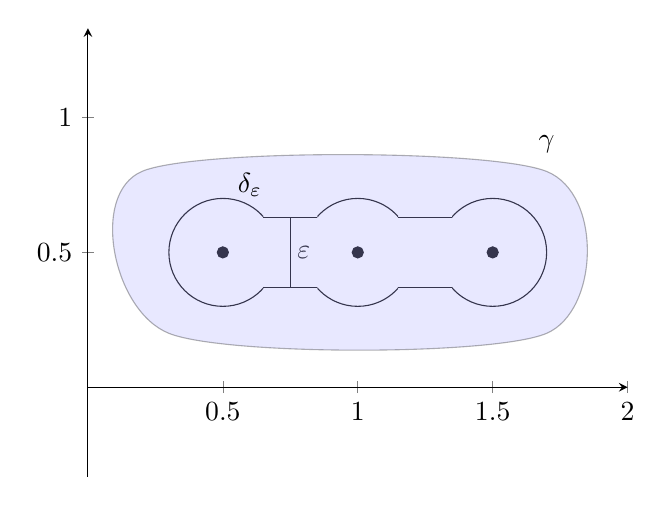
\begin{tikzpicture}
            \begin{axis}[
                axis equal,
                axis lines=center,
                xmin=0, xmax=2,
                ymin=0, ymax=1,
            ]

                \begin{scope}
                    \clip (0, 0) rectangle (0.65, 1);
                    \draw (0.5, 0.5) circle (0.2);
                    \filldraw (0.5, 0.5) circle (2pt);
                \end{scope}

                \draw (0.65, 0.63) -- (0.85, 0.63);
                \draw (0.65, 0.37) -- (0.85, 0.37);

                \begin{scope}
                    \clip (0.85, 0) rectangle (1.15, 1);
                    \draw (1, 0.5) circle (0.2);
                    \filldraw (1, 0.5) circle (2pt);
                \end{scope}
                
                \draw (1.15, 0.63) -- (1.35, 0.63);
                \draw (1.15, 0.37) -- (1.35, 0.37);

                \begin{scope}
                    \clip (1.35, 0) rectangle (2, 1);
                    \draw (1.5, 0.5) circle (0.2);
                    \filldraw (1.5, 0.5) circle (2pt);
                \end{scope}

                \draw (0.75, 0.37) -- (0.75, 0.63);
                \node at (0.8, 0.5) {$\varepsilon$};

                \draw[fill=blue!30, opacity=0.3] plot[smooth cycle] coordinates {(0.3, 0.2) (1.7, 0.2) (1.7, 0.8) (0.2, 0.8)};
                \node at (1.7, 0.9) {$\gamma$};
                \node at (0.6, 0.75) {$\delta_\varepsilon$};
            \end{axis}
        \end{tikzpicture}
    \end{figure}
    \noindent As $\varepsilon \to 0$, we get circles centered at the isolated points. This implies that
    \[\oint_\gamma f(z) \ dz = \oint_{\delta_\varepsilon} f(z) \ dz \to 2\pi i \sum_{n=1}^k \operatorname{res}(f, c_n)\]
    as $\varepsilon \to 0$ by Cauhy's integral formula.
\end{proof}

Now, we will look at computing residues.
\begin{proposition}
    If $f: \Omega \setminus \{c\} \to \mathbb{C}$ is holomorphic and has a pole of order $m$ at $c \in \Omega$, then
    \[\operatorname{res}(f, c) = \frac{1}{(m-1)!} \lim_{z \to c} \frac{d^{m-1}}{dz^{m-1}} \left((z - c)^m f(z)\right).\]
\end{proposition}
\begin{proof}
    We know that $g: \Omega \to \mathbb{C}$ given by $g(z) = (z - c)^m f(z)$ is holomorphic on $\Omega$. In that case, we can find an open disc $D_c$ centered at $c$ such that
    \[g(z) = a_0 + a_1 (z - c) + a_2 (z - c)^2 + \dots\]
    So, the Laurent series of $f$ is
    \[f(z) = a_0 (z - c)^{-m} + a_1 (z - c)^{-m + 1} + \dots + a_{m-1} (z - c)^{-1} + a_m + \dots\]
    This implies that
    \begin{align*}
        \operatorname{res}(f, c) &= a_{m-1} \\
        &= \frac{g^{(m-1)}(c)}{(m-1)!} \\ % Taylor series
        &= \frac{1}{(m-1)!} \lim_{z \to c} \frac{d^{m-1}}{dz^{m-1}} \left((z - c)^m f(z) \right). % f isn't defined at c, so limit + write in Leibniz notation
    \end{align*}
\end{proof}
\noindent This allows us to compute residues quite easily. An example is given below.
\begin{example}
    The function $f: \mathbb{C} \setminus \{1, e^{2\pi i/3}, e^{4\pi i/3}\} \to \mathbb{C}$ given by
    \[f(z) = \frac{1}{z^3 - 1}\]
    has 
    \[\operatorname{res}(f, c) = \frac{1}{3c^2}\]
    for $c \in \{1, e^{2\pi i/3}, e^{4\pi i/3}\}$.
\end{example}
\begin{proof}
    We find that
    \[z^3 - 1 = (z - 1) (z - e^{2\pi i/3}) (z - e^{4\pi i/3}).\]
    So, $f$ has simple poles at $z = 1$, $z = e^{2\pi i/3}$ and $z = e^{4\pi i/3}$. In that case,
    \begin{align*}
        \operatorname{res}(f, c) &= \frac{1}{0!} \lim_{z \to c} \frac{z - c}{z^3 - 1} \\
        &= \lim_{z \to c} \frac{1}{3z^2} \\
        &= \frac{1}{3c^2}
    \end{align*}
    using L'Hopital's rule.
\end{proof}

% \[\frac{z^2 + 5z + 3}{z(z + 1)^2}\]

% \[\frac{\sin z}{z^6}\]

\begin{example}
    Let $k: \mathbb{C} \setminus \{1, 2, 4\} \to \mathbb{C}$ be given by
    \[k(z) = \frac{1}{z - 1} + \frac{3z + 1}{(z - 2)^2} + \frac{3}{z - 4}.\]
    Then,
    \[\operatorname{res}(k, 1) = 1, \qquad \operatorname{res}(k, 2) = 3, \qquad \operatorname{res}(k, 4) = 3.\]
\end{example}
\begin{proof}
    We have isolated singularities at $z = 1$, $z = 2$ and $z = 4$. Moreover, there are simple poles at $z = 1$ and $z = 4$, and a pole of order 2 of $z = 2$. We find that
    \begin{align*}
        \operatorname{res}(k, 1) &= \lim_{z \to 1} \frac{z-1}{z-1} + \frac{(3z + 1)(z-1)}{(z - 2)^2} + \frac{3(z-1)}{z - 4} \\
        &= \lim_{z \to 1} 1 + \frac{(3z + 1)(z-1)}{(z - 2)^2} + \frac{3(z-1)}{z - 4} = 1,
    \end{align*}
    and
    \begin{align*}
        \operatorname{res}(k, 2) &= \lim_{z \to 2} \frac{d}{dz} \frac{(3z + 1)(z-2)^2}{(z-2)^2} \\
        &= \lim_{z \to 2} \frac{d}{dz} (3z + 1) = 3.
    \end{align*}
    Finally,
    \[\operatorname{res}(k, 4) = \lim_{z \to 4} \frac{3(z-4)}{z - 4} = 3.\]
\end{proof}
So, Cauchy's Residue Theorem tells us that
\[\oint_\gamma k(z) \ dz = 2\pi i (1 + 3) = 8\pi i,\]
where $\gamma$ is centered at $0$ with radius $R \in (2, 4)$. Instead, if $R > 4$, Cauchy's Residue Theorem tells us that
\[\oint_\gamma k(z) \ dz = 2\pi i (1 + 3 + 3) = 14\pi i.\]

\subsection{Improper integrals}
We can use residues to compute improper real integrals. We will consider integrals of the form
\[I = \int_{-\infty}^\infty f(x) \ dx.\]
To apply Cauchy's residue theorem, we first need to show that the integral $I$ converges.
\begin{proposition}
    Let $f: \Omega \to \mathbb{C}$ be a complex-valued function with $\mathbb{R} \subseteq \Omega$ such that $z^2 f(z)$ is bounded for large values of $|z|$. Then, the integral
    \[\int_{-\infty}^\infty f(x) \ dx\]
    converges.
\end{proposition}
\begin{proof}
    Since $z^2 f(z)$ is bounded, there exists an $M > 0$ such that $|z^2 f(z)| \leq M$ for large values of $|z|$. In that case, we find that for large $x \in \mathbb{R}$,
    \[|f(x)| \leq \frac{M}{|x|^2} \leq \frac{1}{1 + x^2}.\]
    We know that
    \[\int_{-\infty}^\infty \frac{1}{1 + x^2} = \lim_{R \to \infty} \left[\tan^{-1}(x)\right]_{-R}^{R} = \lim_{R \to \infty} 2\tan^{-1}(R) = \pi.\]
    So, by comparison, we find that the integral $I$ converges.
\end{proof}

We will use this result to compute some integrals.
\begin{example}
    The integral 
    \[\int_{-\infty}^\infty \frac{1}{(x^2 + 1)(x^2 + 4)} \ dx = \frac{\pi}{6}.\]
\end{example}
\begin{proof}
    Let
    \[f(z) = \frac{1}{(z^2 + 1)(z^2 + 4)} = \frac{1}{(z - i)(z + i)(z - 2i)(z + 2i)}.\]
    For $R > 2$, let
    \[I_R = \int_\gamma f(z) \ dz,\]
    where $\gamma$ is the boundary of the upper half of the disc with center $0$ and radius $R$. There are no singularities of $f$ on $\gamma$, and the singularities inside $\gamma$ are at $i$ and $2i$. Moreover, both the singularities are poles of order $1$. In that case,
    \begin{align*}
        \operatorname{res}(f, i) &= \lim_{z \to i} \frac{z - i}{(z - i)(z + i)(z - 2i)(z + 2i)} \\
        &= \frac{1}{(i + i)(i - 2i)(i + 2i)} = \frac{1}{6i},
    \end{align*}
    and
    \begin{align*}
        \operatorname{res}(f, 2i) &= \lim_{z \to 2i} \frac{z + 2i}{(z - i)(z + i)(z - 2i)(z + 2i)} \\
        &= \frac{1}{(2i + i)(2i - i)(2i + 2i)} = -\frac{1}{12i}.
    \end{align*}
    So, Cauchy's residue theorem tells us that
    \[I_R = 2\pi i \left(\frac{1}{6i} - \frac{1}{12i}\right) = \frac{\pi}{6}.\]
    \begin{figure}[H]
        \centering
        \begin{tikzpicture}
            \centering
            \begin{axis}[
                axis lines=center,
                axis equal,
                xmax=3, xmin=-3,
                ymax=3, ymin=0,
                xticklabels={$-R$, $R$},
                xtick={-2.5, 2.5},
                yticklabels={$i$, $2i$, $R$},
                ytick={2/3, 4/3, 2.5},
            ]
                \draw[red, thick] (2.5, 0) arc (0:180:2.5);
                \draw[->, thick, red] (-1.95, 1.56) -- (-2, 1.5);
                
                \draw[blue, thick] (-2.5, 0) -- (2.5, 0);
                \draw[->, thick, blue] (-1, 0) -- (-0.5, 0);
                
                \node at (2, 2) {$\gamma^+$};
                \node at (0.3, -0.2) {$\gamma$};

                \draw[fill=blue] (0, 2/3) circle (2pt);
                \draw[fill=blue] (0, 4/3) circle (2pt);
            \end{axis}
        \end{tikzpicture}
    \end{figure}
    \noindent The semicircle part $\gamma^+$ has length $\pi R$. In that case, the absolute value along $\gamma^+$ is at most
    \[\pi R \max_{|z| = R} |f(z)|.\]
    Since $|f(z)|$ is approximately $\frac{1}{R^4}$ for large $R$, we find that 
    \[\pi R \max_{|z| = R} |f(z)| \approx \frac{\pi}{R^2} \to 0\]
    as $R \to \infty$. The integral along the straight line part is
    \[\int_{-R}^R f(x) \ dx\]
    tends to the integral
    \[\int_{-\infty}^\infty \frac{1}{(x^2 + 1)(x^2 + 4)} \ dx.\]
    Moreover, 
    \[z^2 f(z) = \frac{z^2}{(z^2 + 1)(z^2 + 4)} = \frac{1}{(1 + 1/z^2)(z^2 + 4)}.\]
    So, $z^2 f(z)$ is bounded for large values of $|z|$. This implies that the integral converges, with
    \[\int_{-\infty}^\infty \frac{1}{(x^2 + 1)(x^2 + 4)} \ dx = \frac{\pi}{6}.\]
\end{proof}
\newpage

\section{Conformal Maps}
We saw previously that a holomorphic function preserves $90^{\circ}$ angles over the map. Now, we show that if $f: \Omega \to \mathbb{C}$ is holomorphic with $f' \neq 0$ on $\Omega$, then the angle between any two curves $\gamma_1, \gamma_2 \subseteq \Omega$ that intersect is preserved. We call such maps conformal.
\begin{definition}
    Let $\Omega \subseteq \mathbb{C}$ be open and let $\gamma_1, \gamma_2 : [0, 1] \to \Omega$ be two paths which intersect at $z = \gamma_1(t_1) = \gamma_2(t_2)$ with $t_1, t_2 \in [0, 1]$. If $\gamma_1'(t_1), \gamma_2'(t_2) \neq 0$, then 
    \[\theta = \operatorname{arg}\left(\frac{\gamma_1'(t_1)}{\gamma_2'(t_2)}\right)\]
    is the \emph{angle} between the tangent vectors. We say that a holomorphic function $f: \Omega \to \mathbb{C}$ is \emph{conformal} at $z$ if the tangent vectors of $f \circ \gamma_1$, $f \circ \gamma_2$ at $w = f(z)$ also have the angle $\theta$ between them.
\end{definition}

We now show that any holomorphic function with a non-zero derivative is conformal.
\begin{proposition}
    If $f: \Omega \to \mathbb{C}$ is differentiable at $z \in \Omega$ and $f'(z) \neq 0$, then $f$ is conformal at $z$.
\end{proposition}
\begin{proof}
    By the chain rule, we find that
    \[\frac{(f \circ \gamma_1)'(t_1)}{(f \circ \gamma_2)t_2} = \frac{f'(\gamma_1(t_1)) \gamma_1'(t_1)}{f'(\gamma_2(t_2)) \gamma_2'(t_2)} = \frac{\gamma_1'(t_1)}{\gamma_2'(t_2)}\]
    since $f'(\gamma_2(t_1)) = f'(\gamma_2(t_2))$. So, the angle between $f \circ \gamma_1$ and $f \circ \gamma_2$ is the same as the angle between $\gamma_1$ and $\gamma_2$.
\end{proof}

Now, we will only consider path connected functions. These are sets such that for any two points $z, w \in U$, there is a path from $z$ to $w$.
\begin{definition}
    Let $U, V \subseteq \mathbb{C}$ be open sets that are path connected. A holomorphic function $f: U \to V$ is \emph{biholomorphic} if it is bijective and its inverse $f^{-1}: V \to U$ is holomorphic.
\end{definition}
A biholomorphic function is conformal.
\begin{proposition}
    Let $f: U \to V$ be a biholomorphic function. Then, $f$ is conformal.
\end{proposition}
\begin{proof}
    We find that
    \begin{align*}
        1 &= (f^{-1} \circ f)' (z) \\
        &= f^{-1} (f'(z)) (f^{-1})'(z).
    \end{align*}
    This implies that $f'(z) \neq 0$ for all $z \in U$. This implies that $f$ is conformal by the result above.
\end{proof}

Next, we will define conformal equivalence.
\begin{proposition}
    Let $U, V \subseteq \mathbb{C}$ be path-connected open sets. We say that $U$ and $V$ are \emph{conformally equivalent} if there exists a biholomorphic map $f: U \to V$.
\end{proposition}
\noindent This is an equivalence relation.
% \begin{proposition}
%     % 
% \end{proposition}
% \begin{proof}
    
% \end{proof}

\begin{theorem}
    Let $\Omega, \mathcal{O} \subseteq \mathbb{C}$ be open and path-connected. If $f: \Omega \to \mathcal{O}$ is biholomorphic, then $u: \mathcal{O} \to \mathbb{R}$ is harmonic if and only if $u \circ f: \Omega \to \mathbb{R}$ is harmonic.
\end{theorem}
\begin{proof}
    \hspace*{0pt}
    \begin{itemize}
        \item First, assume that $u: \mathcal{O} \to \mathbb{R}$ is harmonic. Then, we can solve the Cauchy-Riemann equations to find a harmonic conjugate $v$ of $u$, since $\mathcal{O}$ is path-connected. So, there exists a holomorphic function $g: \mathcal{O} \to \mathbb{C}$ such that $g = u + iv$. By the chain rule, we know that the composition $g \circ f: \Omega \to \mathbb{C}$ is holomorphic. So, the real part
        \[\operatorname{Re}(g \circ f) = u \circ f\]
        is harmonic.
    
        \item Now, assume that $u \circ f: \Omega \to \mathbb{R}$ is harmonic. Since $\Omega$ is path connected, there exists a holomorphic function $h: \Omega \to \mathbb{C}$ such that $\operatorname{Re} h = u \circ f$. We know that $f^{-1}: \mathcal{O} \to \Omega$ is holomorphic, so their composition $h \circ f^{-1}: \mathcal{O} \to \mathbb{C}$ is holomorphic. So, the real part
        \[\operatorname{Re}(h \circ f^{-1}) = (u \circ f) \circ f^{-1} = u\]
        is harmonic.        
    \end{itemize}
\end{proof}

\begin{example}
    Let
    \[H = \{z \in \mathbb{C} \mid \operatorname{Im}(z) > 0\}, \qquad D = \{z \in \mathbb{C} \mid |z| < 1\}.\]
    Then, there is a conformal map $f: H \to D$ given by
    \[f(z) = \frac{z - i}{z + i},\]
    with inverse $g: D \to H$ given by
    \[g(w) = \frac{i(1 + w)}{1 - w}.\]
\end{example}
\begin{proof}
    Since $-i \not\in H$, the map $f$ is defined on $H$. Moreover, for all $z = x + iy \in H$,
    \begin{align*}
        f(z) \overline{f(z)} &= \frac{z - i}{z + i} \frac{\overline{z} + i}{\overline{z} - i} \\
        &= \frac{z\overline{z} + i (z - \overline{z}) + 1}{z\overline{z} - i(z - \overline{z}) + 1} \\
        &= \frac{x^2 + y^2 + 2y + 1}{x^2 + y^2 - 2y + 1} \\
        &= \frac{x^2 + (y + 1)^2}{x^2 + (y - 1)^2}.
    \end{align*}
    Since $y > 0$, we find that $-2y < 2y$. So,
    \[(y - 1)^2 < (y + 1)^2,\]
    meaning that
    \[|f(z)|^2 = \frac{x^2 + (y + 1)^2}{x^2 + (y - 1)^2} < 1.\]
    This implies that $f(z) \in H$. So, $f$ is well-defined.

    Moreover, since $1 \not\in D$, the map $f^{-1}$ is defined on $D$. Moreover, for all $w = x + iy \in H$,
    \begin{align*}
        g(w) &= \frac{i(1 + w)}{1 - w} \\
        &= \frac{i(1 + w)}{1 - w} \frac{1 - \overline{w}}{1 - \overline{w}} \\
        &= \frac{i(1 + w - \overline{w} - w\overline{w})}{1 - w - \overline{w} + w\overline{w}} \\
        &= \frac{i(1 + 2yi - x^2 - y^2)}{1 - 2x + x^2 + y^2} \\
        &= \frac{i - 2y - (x^2 + y^2)}{(x - 1)^2 + y^2}.
    \end{align*}
    In that case,
    \[\operatorname{Im} (g(w)) = \frac{1 - (x^2 + y^2)}{(x- 1)^2 + y^2}.\]
    Since $|z|^2 = x^2 + y^2 < 1$, we find that $g(w) \in H$. So, $g$ is well-defined.
    
    Finally, we find that for all $z \in H$,
    \begin{align*}
        g(f(z)) &= g \left(\frac{z - i}{z + i}\right) \\
        &= \frac{i \left(1 + \frac{z - i}{z + i}\right)}{1 - \frac{z - i}{z + i}} \\
        &= \frac{i(z + i + z - i)}{z + i - (z - i)} \\
        &= \frac{i(2z)}{2i} = z.
    \end{align*}
    Moreover, for all $w \in D$,
    \begin{align*}
        f(g(w)) &= f \left(\frac{i(1 + w)}{1 - w}\right) \\
        &= \frac{\frac{i(1 + w)}{1 - w} - i}{\frac{i(1 + w)}{1 - w} + i} \\
        &= \frac{i(1 + w - (1 - w))}{i(1 + w + 1 - w)} \\
        &= \frac{i(2w)}{2i} = w.
    \end{align*}
    This implies that $f^{-1} = g$. Since both $f$ and $f^{-1}$ are holomorphic, we find that $f$ is a conformal map.
\end{proof}

\end{document}
